\chapter{Realizing a Two-Qubit Processor} \label{chapter:design}

This chapter discusses in depth the design process for the realization of the 2-qubit processor which was used in this work. We will start by introducing the general constraints we face when designing a two-qubit processor, followed by a component-wise discussion of the individual parts of the processor and the associated parameters we need to choose.

\section{Introduction \& Motivation}

\begin{figure}[ht!]
  \centering
	\includegraphics[width=1.\textwidth]{"./material/figures/2-qubit-processor/processor schematic"}
	\caption[Circuit schematic of the two-qubit processor]{The circuit schematic of the two-qubit processor used in this work. Shown are the two Transmon qubits in green, the drive and readout circuit in blue, the fast flux lines in red and the coupling capacitance in magenta.}
	\label{fig:2_qubit_chip_circuit_diagram}
\end{figure}

As discussed in the introduction, the most simple, usable quantum processor contains two qubits that can be manipulated and read out individually and between which one can realize a universal 2-qubit gate. We implement such a two-qubit processor using two Transmon qubits that are coupled by a fixed capacitance and that can be read out out individually by a pair of Josephson bifurcation amplifiers (JBAs). The circuit diagram of our processor is shown in fig. \ref{fig:2_qubit_chip_circuit_diagram}, it shows the two qubits in green, the drive and readout circuit in red, the coupling capacitance between them in magenta and the fast flux lines in read. Also shown is the basic microwave setup used for manipulating and reading out the qubits. In the following sections we will discuss each of these components and the parameters we have chosen for them individually.

\subsection{Processor Operation}

\begin{figure}[ht!]
	\centering
	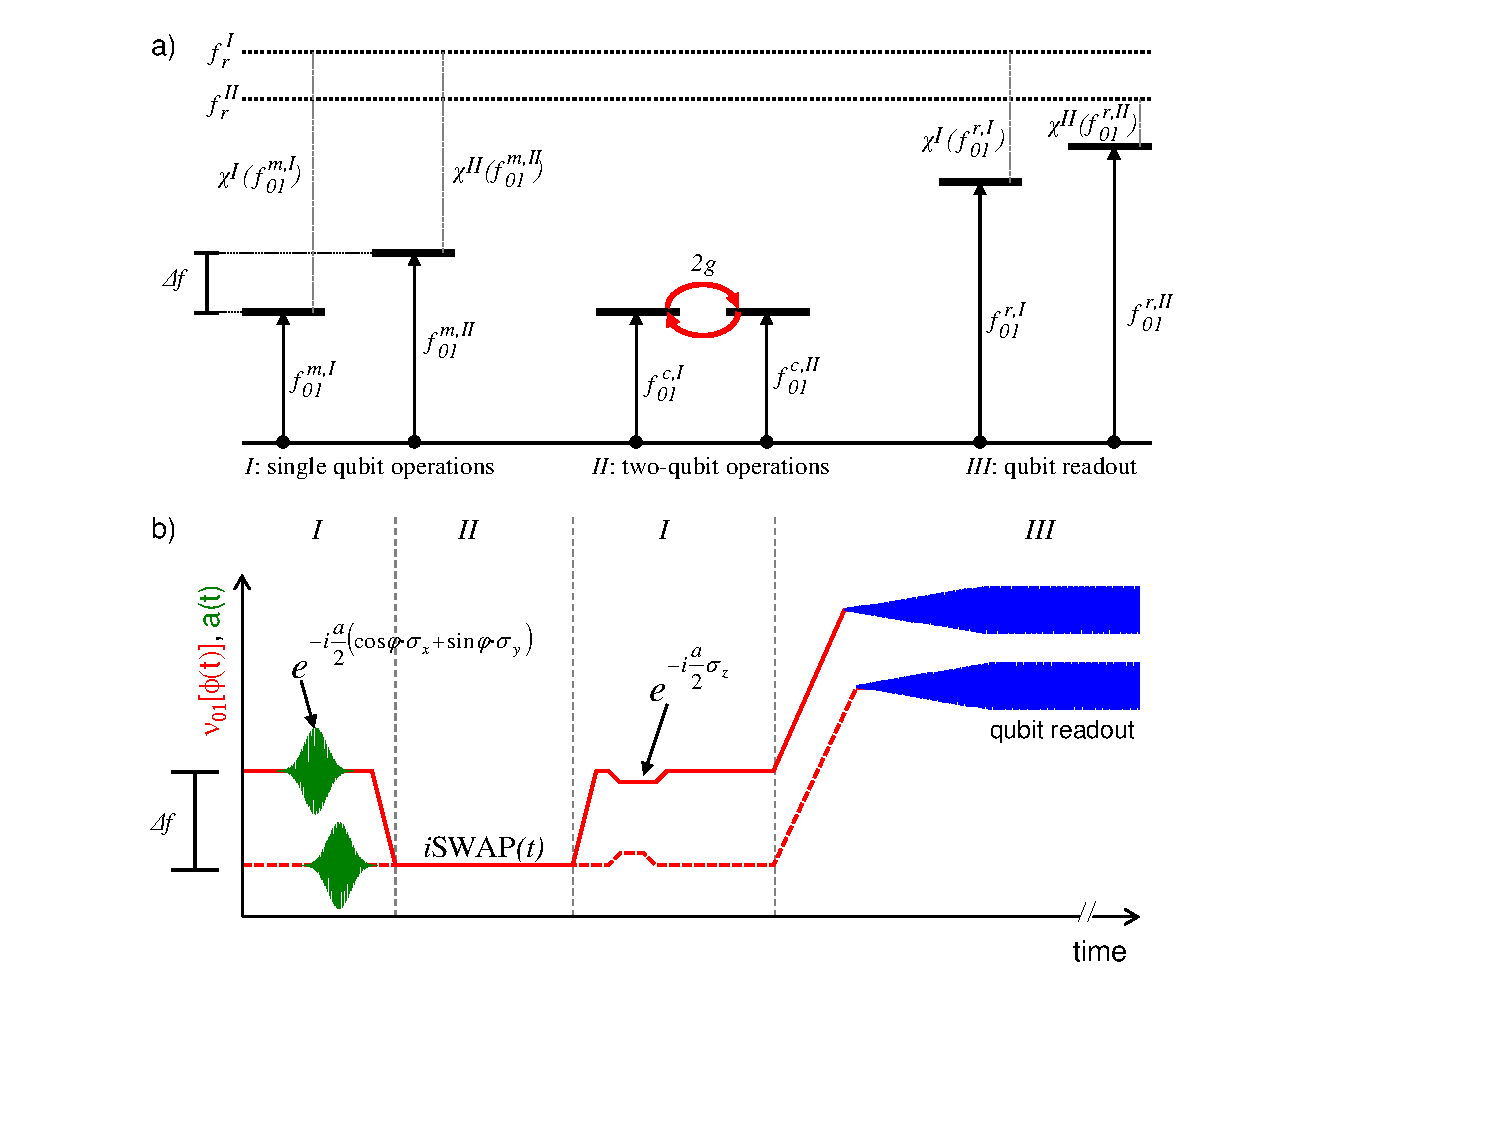
\includegraphics[width=\textwidth]{./material/figures/2-qubit-processor/processor_working_principle}
	\caption[...]{The operation principle of the two-qubit processor. a) The qubit frequencies for different operations. I: Single-qubit manipulation and parking. II: Two-qubit coupling. III: Qubit readout. For each operation, different qubit frequencies are chosen, resulting in different qubit-qubit coupling and qubit-readout couplings $\chi_r^{I,II}(f_{01}^{I,II}$. b) Typical gate sequence illustrating the different operations. The sequence starts with two single-qubit XY-gates, a two-qubit $i\mathrm{SWAP}(t)$ gate, two single-qubit Z-gates and ends with the qubit readout.}
	\label{fig:processor_operation}
\end{figure}

Fig. \ref{fig:processor_operation} illustrates the basic operating principle of the two-qubit processor. We distinguish between three different qubit operations: Single-qubit gates, a two-qubit gate and qubit readout. For each of these operations, we chose a different set of qubit frequencies $f_{01}^{I,II}$. For the single-qubit gates, the two frequencies $f_{01}^{m,I}$ and $f_{01}^{m,II}$ are detuned by $\Delta f_m = f_{01}^{m,II}-f_{01}^{m,I}$. This tuning is chosen such that no effective qubit-qubit is present, as we explain later. Furthermore, the detuning between each qubit and its readout resonator is such that the qubit lifetime is not limited by the Purcell effect as given in eq. (). To realize a two qubit gate, we tune the two qubits in resonance such that $f_{01}^{c,I} = f_{01}^{c,II}$. At this point, the qubits experience a swapping interaction as given in eq. (\ref{eq:cqed_qubit_interaction_hamiltonian}) with a swapping frequency $2g$. For the readout, we choose the qubit frequencies $f_{01}^{r,I}$, $f_{01}^{r,II}$ such that the corresponding dispersive shifts $\chi^I(f_{01}^{r,I})$ and $\chi^{II}(f_{01}^{r,II})$ provide optimal readout visibility.

\section{Qubit Design}

For the qubits, the main design goal is high coherence time, good frequency tunability and the possibility of fast qubit driving. The coherence time of the qubits is limited by relaxation to the ground state and dephasing due to coupling to external noise sources. The dephasing of the qubit state is caused mainly by noise-induced fluctuations of the qubit frequency, which we will discuss in the next section. The relaxation is caused mainly by the coupling of the Transmon to its environment and by internal losses inside the Josephson junctions and the capacitor of the qubit. 

Frequency tunability is important since it will allow us to implement two-qubit gates and to position the qubit ideally for readout or manipulation, as will be explained later. However, strongly coupling the qubit to a fast flux line can induce relaxation and dephasing as well. In the following sections we discuss therefore which coupling strength is adequate and how much the flux coupling contributes to the decoherence time of the qubit.

The drive speed of the qubit --i.e. the frequency at which we can drive qubit transitions-- is ultimately limited by its anharmonicity. When the drive frequency becomes comparable to the anharmonicity we start to induce transitions to higher Transmon levels, therefore ``leaking'' out of the computational basis and producing unitary errors. As we will see, the anharmonicity of the Transmon cannot be chosen arbitarily high since the sensitivity of the Transmon to charge noise increases exponentially with its anharmonicity, it is therefore necessary to find a compromise.

We will start our discussion of the qubit design by discussing the choice of the following qubit parameters:

\begin{enumerate}
\item The maximum qubit transition frequency $f_{01}$
\item The qubit anharmonicity $\alpha$
\item The qubit critical current asymmetry $d$
\item The size of the qubit flux loop and its coupling to the fast flux line
\end{enumerate}

\subsection{Qubit Transition Frequency and Anharmonicity}

The maximum transition frequency $f_{01}^0 = \sqrt{E_J E_C/2}/h$ \todo{verify constants!} of the qubit should be chosen in function of the readout resonator frequency such that it is possible to tune the two of them sufficiently close, thereby achieving the optimal readout fidelity. Chosing a qubit frequency above the cavity frequency should therefore be avoided, since it implies a stronger flux dependence of the qubit frequency at frequencies below the resonator frequency, thus increasing qubit dephasing when operating the qubit there. Hence, ideally the maximum qubit frequency should be chosen such that it corresponds to the optimal frequency for the qubit readout, as will be discussed later.

\smallskip

The anharmonicity $\alpha_r=-(8E_J/E_C)^{-1/2}$ of the qubit can be tuned by changing the ratio of charging and Josephson energy $E_J/E_C$. In general, one aims to have as much anharmonicity as possible in order to avoid inducing leakage to higher level of the quantum system when driving the qubit at high transition frequencies. On the other hand, increasing the anharmonicity (and thus decreasing $E_J/E_C$) will also lead to more charge-induced dephasing of the qubit, thus limiting the coherence time. For our setup, we chose an anharmonicity of the order of $-240\;\mathrm{MHz}$ which allows us to perform single qubit gates at $\approx 100 \;\mathrm{MHz}$ transition frequency without inducing too much leakage to the higher qubit states (a detailed analysis of this leakage will be given in the main section of this thesis). 

\smallskip

Given $f_{01}^0$ and $\alpha_r$ (or equivalently $\alpha$), we can calculate the required charging and Josephson energies of our qubit easily as
%
\begin{eqnarray}
E_C & = & -\alpha \\
E_J & = & \frac{(4\pi\hbar f_{01}^0)^2}{|\alpha|}
\end{eqnarray}
%
For our processor, we chose values $f_{01}^0=7.0\;\mathrm{GHz}$ and $\alpha=-240\;\mathrm{MHz}$, respectively, which yields a Josephson energy $E_J=$ and a charging energy $E_C=$.

\smallskip

We can estimate the dpehasing time of the qubit as a function of these energies by using an equation given in \cite{koch_charge-insensitive_2007}:
%
\begin{equation}
T_2 \simeq \frac{\hbar}{A}\left|\frac{\partial E_{01}}{\partial n_g}\right|^{-1} \simeq \frac{\hbar}{A\pi |\epsilon_1|}
\end{equation}
%
where $A$ is an empirical parameter and $\epsilon_m$ depends exponentially on $E_J/E_C$ and is given as
%
\begin{equation}
\epsilon_m \simeq (-1)^m E_C \frac{2^{4m+5}}{m!}\sqrt{\frac{2}{\pi}}\left(\frac{E_J}{2E_C}\right)^{m/2+3/4}e^{-\sqrt{8 E_J / E_C}}
\end{equation}
%
The dephasing time of the qubit is thus increasing exponentially with the ratio $E_J/E_C$ if $E_J \gg E_C$, whereas the anharmonicity decreases only geometrically with $E_J/E_C$. For our values of $E_J$ and $E_C$ and for a value $A=$, we obtain a dephasing time $T_2=$.

\subsection{Qubit Critical Current Asymmetry}

The critical current asymmetry of the qubit SQUID determines the modulation depth of the transition frequency as a function of the flux applied to the SQUID loop. The interest of choosing a non-zero $d$ (and thus a reduced frequency modulation depth) is to reduce the flux-induced dephasing of the qubit state, which is given as \citep{koch_charge-insensitive_2007}
%
\begin{equation}
T_2 = \frac{\hbar}{A}\left|\frac{\partial E_{01}}{\partial \Phi}\right|^{-1}
\end{equation}
%
where $A$ is an emperical parameter. Hence, the coherence rate increases proportional to the derivative of the qubit energy as a function of the applied flux. On the other hand, cricital current asymmetries can open additional relaxation channels \citep{} such that the overall effect of increasing $d$ is not necessarily monotonous. For our qubits, we chose values of the asymmetry of $d_{I}=0.2$ and $d_{II}=0.35$. However, as we will show later this choice did not led to increased dephasing times of the qubits and should generally be avoided.\todo{cite relevant sections of the Koch paper!}

\subsection{Coupling of the Qubit to the Fast Flux Line}

\begin{SCfigure}
\centering
	\includegraphics[width=6cm]{"./material/figures/2-qubit-processor/fluxline design"}
	\caption[]{Image of the fast flux line used in our 2-qubit processor. The fluxline is separated from the qubit SQUID loop through a stretch of ground plane, the seperation between the fluxline and the qubit is $\approx 20\;\mathrm{\mu m}$. The flux coupling coefficient is given as $1\Phi_0/20\;\mathrm{mA}$.}
	\label{fig:fluxline_design}
\end{SCfigure}

Another critical parameter to chose is the coupling of the qubit the fast flux line. This coupling must be sufficiently strong to allow large frequency displacements of the qubit during operation of the processor but not so strong as to induce additional qubit relaxation or dephasing. A comprehensive summary of fluxline-induced dephasing and relaxation mechanism can be found in \cite{koch_charge-insensitive_2007}. For our qubit chip, we chose a geometry as depicted in fig. \ref{fig:fluxline_design}. Here, the distance between the qubit SQUID loop and the flux line is approx. $20\;\mathrm{\mu m}$, thus the flux coupling to the qubit is given as approx. $1 \Phi_0 / 20\;\mathrm{mA}$. The capacitive coupling between the qubit electrodes and the fluxline is $C_{qf}=??\;\mathrm{fF}$. This capacitive coupling yields an additional contribution to the qubit relaxation rate of the order of $\Gamma_{qf}\approx$. \todo{add more info on the relevant relaxation}.

\subsection{Qubit-Qubit Coupling}

To realize universal two-qubit gate operations it is necessary to provide a kind of coupling between the two qubits of our processor. As discussed before, we use direct capacitive coupling to achieve this for our processor. The coupling strength $g_{qq}$ between the two qubits can be calculated by using eq. (\ref{eq:cqed_capacitive_coupling}). This coupling strength must be chosen such that the interaction between the qubits is sufficiently fast to realize two-qubit gate operations with adequate fidelity but not too strong in order to still allow us to controllably switch on and off the coupling by detuning the qubit frequencies. In general, by diagonalizing the Hamiltonian given in eq. (\ref{eq:cqed_qubit_interaction_hamiltonian}) we find for the swapping frequency $f_{qq}$ and the swap amplitude $a_{qq}$ of the two coupled qubits as a function of the qubit-qubit detuning $\Delta=f_{01}^I-f_{01}^{II}$ the values
%
\begin{eqnarray}
f_{qq} & = & \frac{1}{2}\sqrt{16g^2+\Delta^2} \notag \\
a_{qq} & = & \frac{4g}{\sqrt{16g^2+\Delta^2}} \label{eq:qubit_coupling_amplitude_and_frequency}
\end{eqnarray}
%

\begin{figure}[ht!]
	\centering
	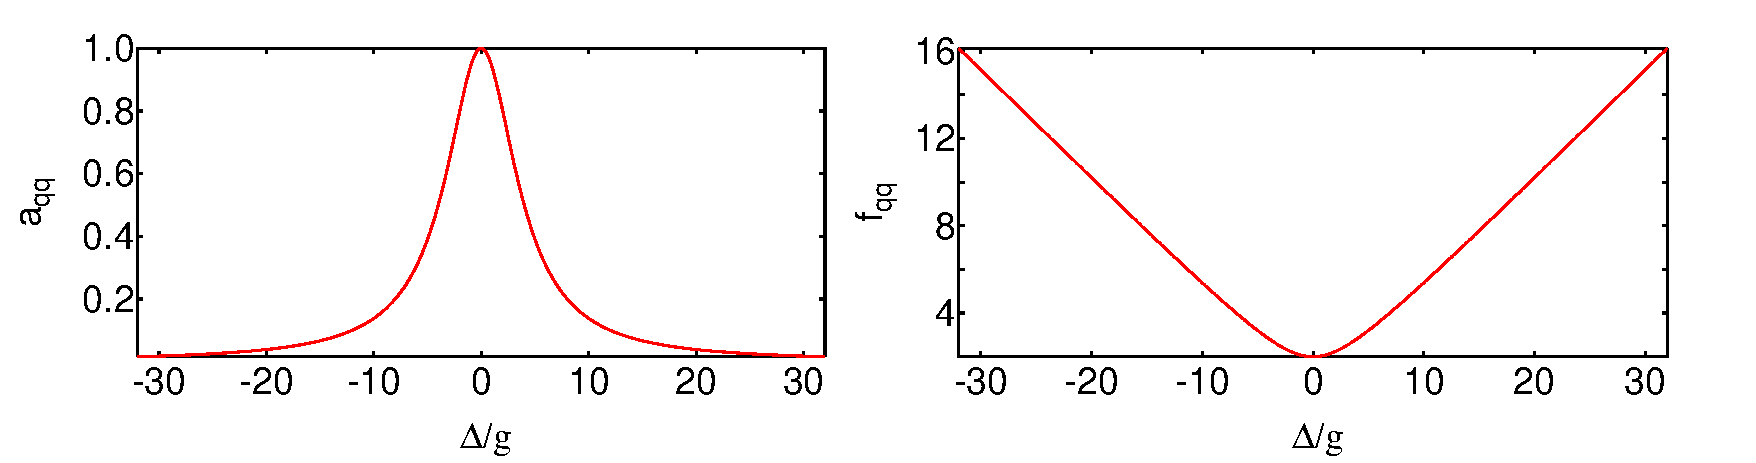
\includegraphics[width=1\textwidth]{./material/mathematica/qubit_coupling_amplitude_and_frequency}
	\caption[]{The swapping amplitude $a_{qq}$ and frequency $f_{qq}$ as given by eq. (\ref{eq:qubit_coupling_amplitude_and_frequency}). For $\Delta \gg g$, the amplitude of the swap decreases $\propto 1/\Delta$ and the frequency increases $\propto \Delta$. To effectively switch of the qubit-qubit level below the 1 \% error level, a detuning of $\Delta \approx 40 g$ is required.}
	\label{fig:qubit_coupling_amplitude_and_frequency}
\end{figure}

Fig. \ref{fig:qubit_coupling_amplitude_and_frequency} shows this amplitude and frequency as a function of the normalized qubit-qubit detuning $\Delta/g$. As can be seen, for $\Delta \gg g$ the swap amplitude decreases $\propto 1/\Delta$ whereas the swap frequency increases $\propto \Delta$. To turn off the qubit-qubit coupling below the 1 \% level it is necessary to detune the qubits by $\Delta \approx 40 g$. It is therefore important to choose $g$ such that it is possible to tune the qubits in and out of resonance sufficiently fast in order to realize a reliable two-qubit gate and switch of the qubit-qubit interaction if wanted. For our processor, we chose $2g = 10\;\mathrm{MHz}$, hence we need to detune the qubits by only $200\;\mathrm{MHz}$ to switch off the coupling between them, which is easily achievable using our fast flux lines. In resonance, the swap frequency of $100\;\mathrm{MHz}$ allows us to realize an $\sqrt{i\mathrm{SWAP}}$ gate in $25\;\mathrm{ns}$ and an $i\mathrm{SWAP}$ gate in $50\;\mathrm{ns}$, which is sufficiently fast compared to the estimated relaxation and dephasing times of the qubits.
\section{Readout Design}

In the following section we discuss the design of the qubit readout. The main parameters that we need to choose for the readout are

\begin{enumerate}
\item The frequency $\omega_r$, quality factor $Q$ and nonlinearity $K$ of the readout resonator
\item The coupling $g_{qr}$ between the qubit and the readout resonator
\end{enumerate}

The frequency $f_r$ of the resonator is chosen high enough to have a negligibly low thermal photon occupation probability at the operating temperature $T=20\;\mathrm{mK}$ of our experiment. Also, the choice of frequency is limited by the availability of sufficiently good cryogenic microwave components (especially circulators) in the chosen frequency band. For our qubit processor, we chose resonator frequencies of $f_r^I = 6.7\;\mathrm{GHz}$ and $f_r^{II}=7.85\;\mathrm{GHz}$. The resonance frequencies of the two resonators are detuned by $150\;\mathrm{MHz}$ in order to reduce the effect of unwanted microwave crosstalk between them.

\smallskip

The other relevant parameters of the readout resonator are its quality factor $Q$ and its Kerr constant $K$. The choice of the quality factor influences the relaxation rate of the qubit through the Purcell effect as well as the rate at which photons can be created in or extracted from the resonator, which in turn also determines the speed of the qubit readout. A comprehensive review of the interplay between qubit relaxation, readout speed and readout fidelity can be found in \cite{mallet_single-shot_2009}. To quantify the Purcell relaxation of the qubit trough the readout resonator we can use an equation given in \citep{koch_charge-insensitive_2007}:
%
\begin{equation}
\gamma_k^{(i,i+1)} = \kappa \frac{g_{i,i+1}^2}{(\omega_{i,i+1}-\omega_r)^2}
\end{equation}
%
Here, $\omega_r$ is the frequency of the readout resonator, $\omega_{i,i+1}$ is the $\ket{i}\to\ket{i+1}$ transition frequency of the Transmon and $g_{i,i+1}$ is the qubit-resonator coupling strength for this transition. As can be seen, the Purcell relaxation rate decreases quadratically with the qubit-resonator detuning and increases quadratically with the qubit-resonator coupling strength $g_{i,i+1}$\todo{choose consistent notation, e.g. $g_{qr}^{i,i+1}$!}. For our resonators, we chose $Q=800$ which yields $\kappa_I = 52.6\;\mathrm{MHz}$ and $\kappa_{II} = 53.8\;\mathrm{MHz}$. Thus, for the above quality factors, a qubit-resonator coupling $2g_{qr}^{01}=2\pi \cdot 50\;\mathrm{MHz}$ and a detuning of $\omega_{01}-\omega_r = 2\pi \cdot 500 \;\mathrm{MHz}$ we obtain a Purcell relaxation time of $T_{1}^{01} \approx 7.5\;\mathrm{\mu s}$, which is bigger than the intrinsic relaxation time of a typical Transmon qubit by a large factor (however, certain new types of Transmon qubits can surpass this relaxation time).

\smallskip

The choice of the Kerr nonlinearity $K$ determines the number of photons in the low- and high-amplitude oscillation state of the resonator and the size of the ``bifurcation region'' of the JBA. It is important to choose $K$ sufficiently high in order to be able to achieve reliable readout operation. On the other hand, the photons present in the resonator during the readout can induce decoherence in the qubit and will shift its resonance frequency proportional to the number of photons. This frequency shift can create unwanted effects such as recoupling of the two qubits of our processor and should therefore be minimized. Theoretically, the maximum readout fidelity is achieved when the bifurcation point of the resonator is shifted by more than its linewidth, as a function of the qubit state. The linewidth of the switching probability distribution of the JBA as a function of the incident microwave power can be calculated numerically but usually we use experimental values to characterize it. In our case, this measured linewidth in dB was given as $\Delta p = xx\;\mathrm{dB}$. \todo{add more detail about the readout contrast at a given detuning for the chosen set of parameters.}

\section{Processor Fabrication}

We fabricate the processor on a silicon substrate with a 50 nm thermal oxide layer. First, we depose a 150 nm layer of Niobium by magentron sputtering. Afterwards, we spin a photoresist and define an etch mask through optical lithography. Then we dry-etch in a$\mathrm{SF}_6$ plasma, defining the readout resonators, tranmission lines and qubit flux lines on the chip. This optical patterning is performed for the wafer as a whole. Afterwards, we spin a bilayer of MAA/PMMA electron beam resist (with typically $1050\;\mathrm{nm}$ of MMA and $115\;\mathrm{nm}$ of PMMA thickness). Then the wafer gets diced and the qubits and JBA junctions are patterned per chip using electron beam lithography, using a double-angle shadow evaporation technique to define the Josephson junctions and capacitances on the chip. The e-beam resist is then lifted off chemically in an Acetone bath. We characterize the chip optically afterwards. In addition, we place ``twin'' structures of the Transmon qubits and the JBAs on each chip whose normal state resistance we measure at room temperature. Giving the normal-state resistance of a Josephson junction we can calculate the Josephson energy by using the Ambegaokar-Baratoff relation
%
\begin{equation}
E_J = \frac{2\pi^2 \Delta}{R_n h}
\end{equation}
%
,where $E_J = h I_c / 4\pi e$. Furthermore, we perform numerical microwave simulations to extract the values of all relevant capacitances and inductances on the chip, which allows us to calculate all relevant parameters of our qubit chip.

\begin{SCfigure}
	\includegraphics[width=10cm]{"./material/figures/2-qubit-processor/processor photos"}
	\caption{Optical and electron microscope photos of the two-qubit processor realized in this work. a) shows the full processor with the two coupled qubits, fluxlines and readout resonator. b) shows an enlarged version of the central region of the chip with the two qubits and the coupling capacitance. c) Shows a single Transmon qubit.}
	\label{fig:setup_wiring}
\end{SCfigure}

